\documentclass[fleqn,usenatbib]{mnras}

% MNRAS is set in Times font. If you don't have this installed (most LaTeX
% installations will be fine) or prefer the old Computer Modern fonts, comment
% out the following line
%\usepackage{newtxtext,newtxmath}
\usepackage{times}
% Depending on your LaTeX fonts installation, you might get better results with one of these:
% \usepackage{mathptmx}
% \usepackage{txfonts}

% Use vector fonts, so it zooms properly in on-screen viewing software
% Don't change these lines unless you know what you are doing
\usepackage[T1]{fontenc}
\usepackage{ae,aecompl}


%%%%% AUTHORS - PLACE YOUR OWN PACKAGES HERE %%%%%
%\usepackage{epsf}
\usepackage{color}
\usepackage{graphicx}
\usepackage{amsmath}	% Advanced maths commands
\usepackage{amssymb}	% Extra maths symbols
\usepackage{mathrsfs}	% Extra extra math symbols
\usepackage{natbib}
%\usepackage[colorlinks,urlcolor=magenta,citecolor=blue,linkcolor=blue]{hyperref}
\usepackage{multirow}
\usepackage{etoolbox}
\usepackage{listings}

\graphicspath{{./figures/}}

%%%%% AUTHORS - PLACE YOUR OWN COMMANDS HERE %%%%%
%%% Fields %%%
\newcommand{\hdf}{HDF-N}
\newcommand{\hdfn}{HDF-N}
\newcommand{\hdfs}{HDF-S}
\newcommand{\cdfs}{CDF-S}

%%% Telescopes %%%
\newcommand{\hst}{\textit{HST}}
\newcommand{\iras}{\textit{IRAS}}
\newcommand{\iso}{\textit{ISO}}
\newcommand{\spitzer}{\textit{Spitzer}}
\newcommand{\sirtf}{\textit{Spitzer}}
\newcommand{\chandra}{\textit{Chandra}}

%%% Filters %%%
\newcommand{\wfu}{\hbox{$\mathrm{U}_{300}$}}
\newcommand{\wfb}{\hbox{$\mathrm{B}_{450}$}}
\newcommand{\wfv}{\hbox{$\mathrm{V}_{606}$}}
\newcommand{\wfi}{\hbox{$\mathrm{I}_{814}$}}
\newcommand{\acsb}{\hbox{$\mathrm{B}_{435}$}}
\newcommand{\acsv}{\hbox{$\mathrm{V}_{606}$}}
\newcommand{\acsi}{\hbox{$i_{775}$}}
\newcommand{\acsz}{\hbox{$z_{850}$}}
\newcommand{\nicj}{\hbox{$\mathrm{J}_{110}$}}
\newcommand{\nich}{\hbox{$\mathrm{H}_{160}$}}
\newcommand{\wfcy}{\hbox{$\mathrm{Y}_{105}$}}
\newcommand{\wfcj}{\hbox{$\mathrm{J}_{125}$}}
%\newcommand{\wfcj}{\hbox{$J_{110}$}}
\newcommand{\wfch}{\hbox{$\mathrm{H}_{160}$}}
\newcommand{\sdssu}{\hbox{$u$}}
\newcommand{\sdssg}{\hbox{$g$}}
\newcommand{\sdssr}{\hbox{$r$}}
\newcommand{\sdssi}{\hbox{$i$}}
\newcommand{\sdssz}{\hbox{$z$}}
\newcommand{\mone}{\hbox{$[3.6]$}}
\newcommand{\mtwo}{\hbox{$[4.5]$}}
\newcommand{\mthree}{\hbox{$[5.8]$}}
\newcommand{\mfour}{\hbox{$[8.0]$}}
%\newcommand{\mone}{\hbox{$[3.6\mu\mathrm{m}]$}}
%\newcommand{\mtwo}{\hbox{$[4.5\mu\mathrm{m}]$}}
%\newcommand{\mthree}{\hbox{$[5.8\mu\mathrm{m}]$}}
%\newcommand{\mfour}{\hbox{$[8.0\mu\mathrm{m}]$}}

%%% Astronomy Abreviations %%%
\newcommand{\mstar}{\hbox{$\mathrm{M}^\ast$}}
\newcommand{\lstar}{\hbox{$L^\ast$}}
\newcommand{\Msol}{\hbox{$\mathrm{M}_\odot$}}
\newcommand{\msol}{\hbox{$\mathrm{M}_\odot$}}
\newcommand{\Zsol}{\hbox{$Z_\odot$}}
\newcommand{\zsol}{\hbox{$Z_\odot$}}
\newcommand{\Lsol}{\hbox{$L_\odot$}}
\newcommand{\lsol}{\hbox{$L_\odot$}}
\newcommand{\lir}{\hbox{$L_{\mathrm{IR}}$}}
\newcommand{\zph}{\hbox{$z_\mathrm{ph}$}}
\newcommand{\zphot}{\hbox{$z_\mathrm{ph}$}}
\newcommand{\lbol}{\hbox{$L_\mathrm{bol}$}}
\newcommand{\snr}{\hbox{$\mathrm{S/N}$}}
\newcommand{\reff}{\hbox{$r_\mathrm{eff}$}}
\newcommand{\ks}{\hbox{$K_s$}}
\newcommand{\AAA}{\hbox{\AA}}

%%% Spectrum Lines %%%
\newcommand{\lya}{ Ly$\alpha \;$}
\newcommand{\lyb}{Lyman~$\beta$}
\newcommand{\hb}{\hbox{H$\beta$}}
\newcommand{\ha}{\hbox{H$\alpha$}}
\newcommand{\paa}{\hbox{Pa$\alpha$}}

%%% Units %%%
\newcommand{\kms}{\hbox{km~s$^{-1}$}}
\newcommand{\cms}{\hbox{cm~s$^{-1}$}}
\newcommand{\mpc}{\hbox{Mpc$^{-1}$}}
\newcommand{\mpcsq}{\hbox{Mpc$^{-2}$}}
\newcommand{\mpccu}{\hbox{Mpc$^{-3}$}}
\newcommand{\cnts}{\hbox{cnt~s$^{-1}$}} 
\newcommand{\cmsq}{\hbox{cm$^{-2}$}}
\newcommand{\cmcu}{\hbox{cm$^{-3}$}}
\newcommand{\ergscm}{\hbox{erg~s$^{-1}$~cm$^{-2}$}}
\newcommand{\uJy}{\hbox{$\mu$Jy}}
\newcommand{\ujy}{\hbox{$\mu$Jy}}
\newcommand{\degree}{\hbox{$^\circ$}}
\newcommand{\degsq}{\hbox{degree$^2$}}
\newcommand{\arcminsq}{\hbox{arcmin$^2$}}
\newcommand{\um}{\hbox{$\mu$m}}

%%% Math %%%
\newcommand{\lsim}{\lesssim}
\newcommand{\gsim}{\gtrsim}
\newcommand{\mathS}{\hbox{$\mathcal{S}$}}
\newcommand{\mathR}{\hbox{$\mathcal{R}$}}
\newcommand{\mathM}{\hbox{$\mathcal{M}$}}
\newcommand{\mcal}{\hbox{$\mathcal{M}$}}
\newcommand{\rcal}{\hbox{$\mathcal{R}$}}
\newcommand{\scal}{\hbox{$\mathcal{S}$}}
\newcommand{\infinity}{\hbox{$\infty$}}
\newcommand{\err}[2]{$^{+#2}_{-#1}$}

%%% General %%%
\newcommand{\etal}{et al.}
\newcommand{\eg}{e.g.}
\newcommand{\ie}{i.e.}
\newcommand{\cf}{cf.}
% \newcommand{\ion}[2]{\hbox{#1$\;${\small\rm{#2}}}}
\newcommand{\mybullet}{\noindent$\bullet$}
\newcommand{\uit}{\textit{UIT}}
\newcommand{\nd}{...}
%\newcommand{\cmodel}{\hbox{\tt cmodel}}
%\newcommand{\bs}{\hbox{$\!\!\!\!$}}
\newcommand{\todo}[1]{{\tt #1}}
\newcommand{\citeeg}[1]{(\eg, \citealt{#1})}
\newcommand{\ignore}[1]{}

%%% Extra %%% 
% \newcommand{\farcm}{\mbox{\ensuremath{.\mkern-4mu^\prime}}}%fractional arcminute symbol 0.'0
% \newcommand{\farcs}{\mbox{\ensuremath{.\!\!^{\prime\prime}}}}%fractional arcsecond symbol: 0.''0
% \newcommand{\fdg}{\mbox{\ensuremath{.\!\!^\circ}}}%fractional degree symbol:     0.°0
\newcommand{\arcdeg}{\ensuremath{^{\circ}}}%                    % degree symbol:  °
% \newcommand{\sun}{\ensuremath{\odot}}%                          % sun symbol
% \newcommand{\apj}{ApJ}%                                         % Journal abbreviations
% \newcommand{\apjs}{ApJS}
% \newcommand{\apjl}{ApJL}
% \newcommand{\aap}{A{\&}A}
% \newcommand{\aaps}{A{\&}AS}
% \newcommand{\mnras}{MNRAS}
% \newcommand{\aj}{AJ}
% \newcommand{\araa}{ARAA}
% \newcommand{\pasp}{PASP}
\newcommand{\Teff}{\ensuremath{T_{\mathrm{eff}}}}%              % T_eff
\newcommand{\logg}{\ensuremath{\log g}}%                        % log g
\newcommand{\bv}{\ensuremath{B\!-\!V}}%                         % B-V
\newcommand{\ub}{\ensuremath{U\!-\!B}}%                         % U-B
\newcommand{\vr}{\ensuremath{V\!-\!R}}%                         % V-R
\newcommand{\ur}{\ensuremath{U\!-\!R}}%                         % U-R

\newcommand{\editorial}[1]{\textcolor{red}{#1}}

%%%%%%%%%%%%%%%%%%% TITLE PAGE %%%%%%%%%%%%%%%%%%%
\title[Metallicity with CNNs]{Predicting Galaxy Metallicity from Three-Color Images using Convolutional Neural Networks}

% The list of authors, and the short list which is used in the headers.
% If you need two or more lines of authors, add an extra line using \newauthor
\author[Wu and Boada]
{\parbox{\textwidth}{John~Wu$^{1}$\thanks{E-mail: \href{mailto:jw740@physics.rutgers.edu}} and
Steven~Boada$^{1}$}\vspace{0.4cm}\
\\
\parbox{\textwidth}{$^{1}$Physics and Astronomy Department, Rutgers University, Piscataway, NJ 08854-8019, USA\\}}

% These dates will be filled out by the publisher
\date{Accepted XXX. Received YYY; in original form ZZZ}

% Enter the current year, for the copyright statements etc.
\pubyear{2018}

% Don't change these lines
\begin{document}
\label{firstpage}
\pagerange{\pageref{firstpage}--\pageref{lastpage}}
\maketitle

\begin{abstract}
\noindent
Lorem ipsum dolor sit amet, consectetur adipisicing elit, sed do eiusmod tempor incididunt ut labore et dolore magna aliqua. Ut enim ad minim veniam, quis nostrud exercitation ullamco laboris nisi ut aliquip ex ea commodo consequat. Duis aute irure dolor in reprehenderit in voluptate velit esse cillum dolore eu fugiat nulla pariatur. Excepteur sint occaecat cupidatat non proident, sunt in culpa qui officia deserunt mollit anim id est laborum.
\end{abstract}

\section{Introduction}\label{sec:introduction}
Large-area sky surveys, both on-going and planned, are revolutionizing our understanding of galaxy evolution. The on going Dark Energy Survey (DES; \citealt{DES2005}) and planned Large Synoptic Survey Telescope (LSST; \citealt{LSST2012}) will survey vast swaths of the sky and create samples of galaxies much larger than any previously known. Spectroscopic follow-up will be key to a deep understanding of the properties of these galaxies, and constrain galaxy evolution through relations such as the mass-metallicity relation (hereafter MZR; \citealt{Tremonti2004}); or the fundamental metallicity relation, (hereafter FMR; \eg, \citealt{Mannucci2010}). But as the data sets continue to grow, individual galaxy spectroscopic follow-up becomes increasingly impractical.

Fortunately, the large data sets produced are ripe for the application of machine learing (ML) methods. ML is already contributing heavily to wide ranging studies investigating galaxy morphology \citeeg{Dieleman2015, Huertas-Company2015, Beck2018, Dai2018, Hocking2018}, gravitational lensing \citeeg{Lanusse2017, Petrillo2017, Petrillo2018}, galaxy clusters \citeeg{Ntampaka2015, Ntampaka2016}, star-galaxy separation \citeeg{Kim2017}, creating mock galaxy catalogs \citeeg{Xu2013}, and asteroid identification \citeeg{Smirnov2017} among many others.

In recent years, ML methods utilizing learning networks or ``neural'' networks have grown to prominence. While neural networks are a relatively old technique \citeeg{LeCun1989}, their recent increase in popularity is driven by the wide spread availability of cheap graphics processing units (GPUs) which can be used to do general purpose, highly parallel computing. Also, unlike more ``traditional'' ML methods, neural networks excel at image classification and regression problems.

Inferring spectroscopic properties from the imaging taken as part of a large-area photometric survey is, at a basic level, an image regression problem. These problems are most readily solved by use of convolutions in multiple layers of the network (see \eg, \citealt{Krizhevsky2012}). Convolution neural networks (CNNs, or convnets) efficiently learn spatial relations in images whose features are about the same sizes as the convolution filters (or kernels) which are to be learned through training. CNNs are considered \textit{deep} when the number of convolutional layers is large, leading to the term ``deep learning.'' Visualizing their filters reveals that increased depth permits the network to learn more and more abstract features (\eg, from Gabor filters, to geometric shapes, to faces; \citealt{Zeiler2014}).

In this work, we propose to use supervised ML, specifically CNNs, to analyze pseudo-three color images to predict the gas phase metallicity of a sample of galaxies taken as part of a large-area sky survey. We then used the predicted metallicities to recover the well established MZR.

This paper is organized as follows: In Section~\ref{sec:data}, we describe the acquisition and cleaning of the SDSS data sample. In Section~\ref{sec:training} we discuss selection of the network's hyperparameters and outline training the network. We present the main results in Section~\ref{sec:results} and discuss the results in the context of previous works. In Section~\ref{sec:MZR}, we discuss how our recovered MZR compares to other previously known relations. Finally, we summarize our key results and discuss possible future work in Section~\ref{sec:summary}.

Unless otherwise noted, throughout this paper, we use a concordance cosmological model ($\Omega_\Lambda = 0.7$, $\Omega_m = 0.3$, and $H_0= 70$ \kms \permpc), assume a Chabrier initial mass function \citep{Chabrier2003}, use AB magnitudes \citep{Oke1974} and quote uncertainties at the 1-$\sigma$ level.

\section{Data} \label{sec:data}
To create a large training sample, we optically select galaxies from the \textit{Sloan Digital Sky Survey} (SDSS; \citealt{York2000}) DR7 MPA/JHU spectroscopic catalog \citep{Kauffmann2003a, Brinchmann2004, Salim2007}. This catalog provides us with derived spectroscopic properties, stellar mass (\mstar), and gas phase metallicity ($Z$) estimates \citep{Tremonti2004}. We supplement the data from the spectroscopic catalog with photometry in each of the five SDSS photometric bands (\sdssu, \sdssg, \sdssr, \sdssi, \sdssz), along with associated errors from SDSS DR14 \citep{Abolfathi2017}.

We require that galaxies magnitudes are $10 < \sdssu \sdssg \sdssr \sdssi \sdssz < 25$ mag, to avoid saturated, and low signal-to-noise detections. Galaxies should have colors $0 < \sdssu-\sdssr < 6$, to avoid extremely blue or extremely red objects and high confidence ($z_{err} < 0.01$) spectroscopic redshifts greater than $z=0.02$. We also require that the \sdssr-band magnitude measured inside the petrosian radius (petroMag$_r$) be less than 18 mag, corresponding to the spectroscopic flux limit.

With these conditions we construct an initial sample of 142,186 galaxies.

\subsection{SDSS Images}
From this initial sample we create RGB (\sdssi\sdssr\sdssg) image cutouts of each galaxy with the SDSS cutout service\footnote{\url{http://skyserver.sdss.org/dr14/SkyserverWS/ImgCutout/getjpeg}}. Images are scaled to be $128\times128$ pixels in size, corresponding to $15''\times15''$ on the sky. The native $0\farcs396$ SDSS pixel size are rescaled to $0\farcs296$ per pixel.

These RGB JPEG images form the inputs into our network. No further cleaning or filtering of the images is conducted.

\section{Training the Network}\label{sec:training}
%The input layer is simply an image of $128\times 128$ pixels with three channels (RGB).
Before the CNN can be asked to make predictions, it must be trained to learn the relationships between the input data (the images described above) and the desired out put (the metallicity). Once the network is trained we use the test data set to assess the correctness of the predictive relationships.

We split our initial sample of $\sim 140,000$ images into random 60\%, 20\%, and 20\% subsets, which comprise the training, validation, and test data sets respectively. All training images are seen by the network once every training epoch \editorial{what is epoch?}, although usually each epoch is split into a number of mini-batches which are learned in parallel. Mini-batches are usually small \editorial{($\sim256$)} and potentially not representative of the full training sample -- a technique used to prevent overfitting. Overfitting is when the network learns a specific and usually not general set of features which are then misapplied to the test data set.

Each mini-batch is fed forward through the input layers, where a random fraction of connections $p=0.25, 0.50$ \editorial{what?} are removed between each linear layer (a ``dropout''; \citealt{Hinton2012}; see Section~\ref{sec:norm and drop}). When the feed-forward network reports a prediction, a single value or a set of values, then a loss/cost function is used to compute how incorrect the prediction ($\hat y$) is from the true value $y$. We use the root mean squared error (RMSE$~\equiv \sqrt{\langle |\hat y - y|^2\rangle}$) loss function, and seek to minimize it.

We use gradient descent for each mini-batch to adjust each weight parameter, and each fractional contribution of loss is determined by the backpropagation algorithm \citep{LeCun1989}. The backpropagation algorithm is simply the chain rule applied to finite derivatives, and \editorial{skipped?} for any non-linear layers. The gradient is multiplied by the \textit{learning rate} (see Section~\ref{sec:learning rate}); batch-normalization is also applied in addition to a momentum term which ensures that the gradient is itself only changing slowly with each mini-batch. \editorial{what is momentum}

CNNs become difficult to train after many layers are added, likely because the network has already found the best representation possible at a shallower layer, and deeper layers simply noisily propagate the same signal and degrade the loss. To avoid this, we select a network architecture called a residual neural network, or \textit{resnet} \citep{He2016}, which contains enhanced ``shortcut connections'' but is otherwise similar to other CNNs. Resnets have been shown to continue learning with increasing depth without the added cost of extra parameters. \editorial{cite?}
%Therefore resnets are able to learn deep representations of the data.

We use a 34-layer resnet \citep{He2016}, whose architecture consists of three layer groups. Our resnet is initialized to pre-trained weights from the ImageNet data set, which consists of 1.7 million images belonging to 1000 categories of objects found on Earth (\eg, cats, horses, cars, or books). The earlier layer groups generally have already trained filters that represent low-level abstractions, such as edges or Gabor filters, so we first train only the last layer group of the network by ``freezing'' the weights in the first two groups. By reducing the number of trainable parameters, we can rapidly approach the global loss minimum in a few number of epochs.

We train the final layers for two epochs using a learning rate of 0.1, and then ``unfreeze'' the earlier layers and train for another eight epochs using learning rates of [0.001, 0.01, 0.1] for the first, second, and third layer group respectively. For more details about our training methodology, such as the use of learning rate annealing, data augmentation, dropout, batch-normalization, and other hyperparameters, see Section~\ref{sec:learning rate}.

Our training methods near convergence after 10 epochs, and additional training only marginally improves the loss. In total, our training steps requires 25-30 minutes on our GPU and uses under 2~GB of memory (depending on batch size).

%Ensemble methods take $k$ times as long to train.
Prediction using data augmentation (see Section~\ref{sec:data aug}) takes two minutes for our full test set of \editorial{20,466} images, or approximately 6 milliseconds per image (or a little over 1 millisecond per image without augmentation). In comparison, \cite{Huertas-Company2015} train their network for 10 days on a GPU following the Galaxy Zoo architecture.

%Super-convergent training the network takes about 10 hours on a GPU but only yield marginal improvements over the ensemble methods (RMSE~$= 0.0828$ for super-convergent versus $0.0835$ for 5-fold).

We evaluate predictions using not only the RMSE, which approaches the standard deviation for Gaussian-distributed data, but also the NMAD, or the normal median absolute deviation \citeeg{Ilbert2009, Dahlen2013, Molino2017}).
\begin{equation}
{\rm NMAD}(x) \approx 1.4826 \times {\rm median} \big (\big|x - {\rm median }(x) \big|\big ),
\end{equation}
where for a Gaussian-distributed $x$, the NMAD will also approximate the standard deviation, $\sigma$.
NMAD has the distinct advantage in that it is insensitive to outliers for non-Gaussian distributions and is useful for comparing scatter.

% Glossary of terminology:
% \begin{itemize}
% 	\item $Z \equiv 12 + \log ({\rm O/H})$ is the nebular phase metallicity
% 	\item $Z_{\rm true}$ is the spectroscopically derived metallicity
% 	\item $Z_{\rm pred}$ is the CNN predicted metallicity
% 	\item $\Delta Z \equiv Z_{\rm pred} - Z_{\rm true}$ is the residual, or error
% 	\item RMSE~$\equiv \sqrt{\langle |\hat y - y|^2\rangle}$ is the root-mean squared error.
% 	The RMSE loss function is minimized during CNN training.
% 	\item NMAD~$\approx 1.4826 \times {\rm median} \big (\big|x - {\rm median }(x) \big|\big )$ is the normal median absolute deviation
% \end{itemize}

\section{Results}\label{sec:results}
Here we present the galaxy metallicities predicted by our trained network.

\subsection{Example predictions}
\begin{figure*}
	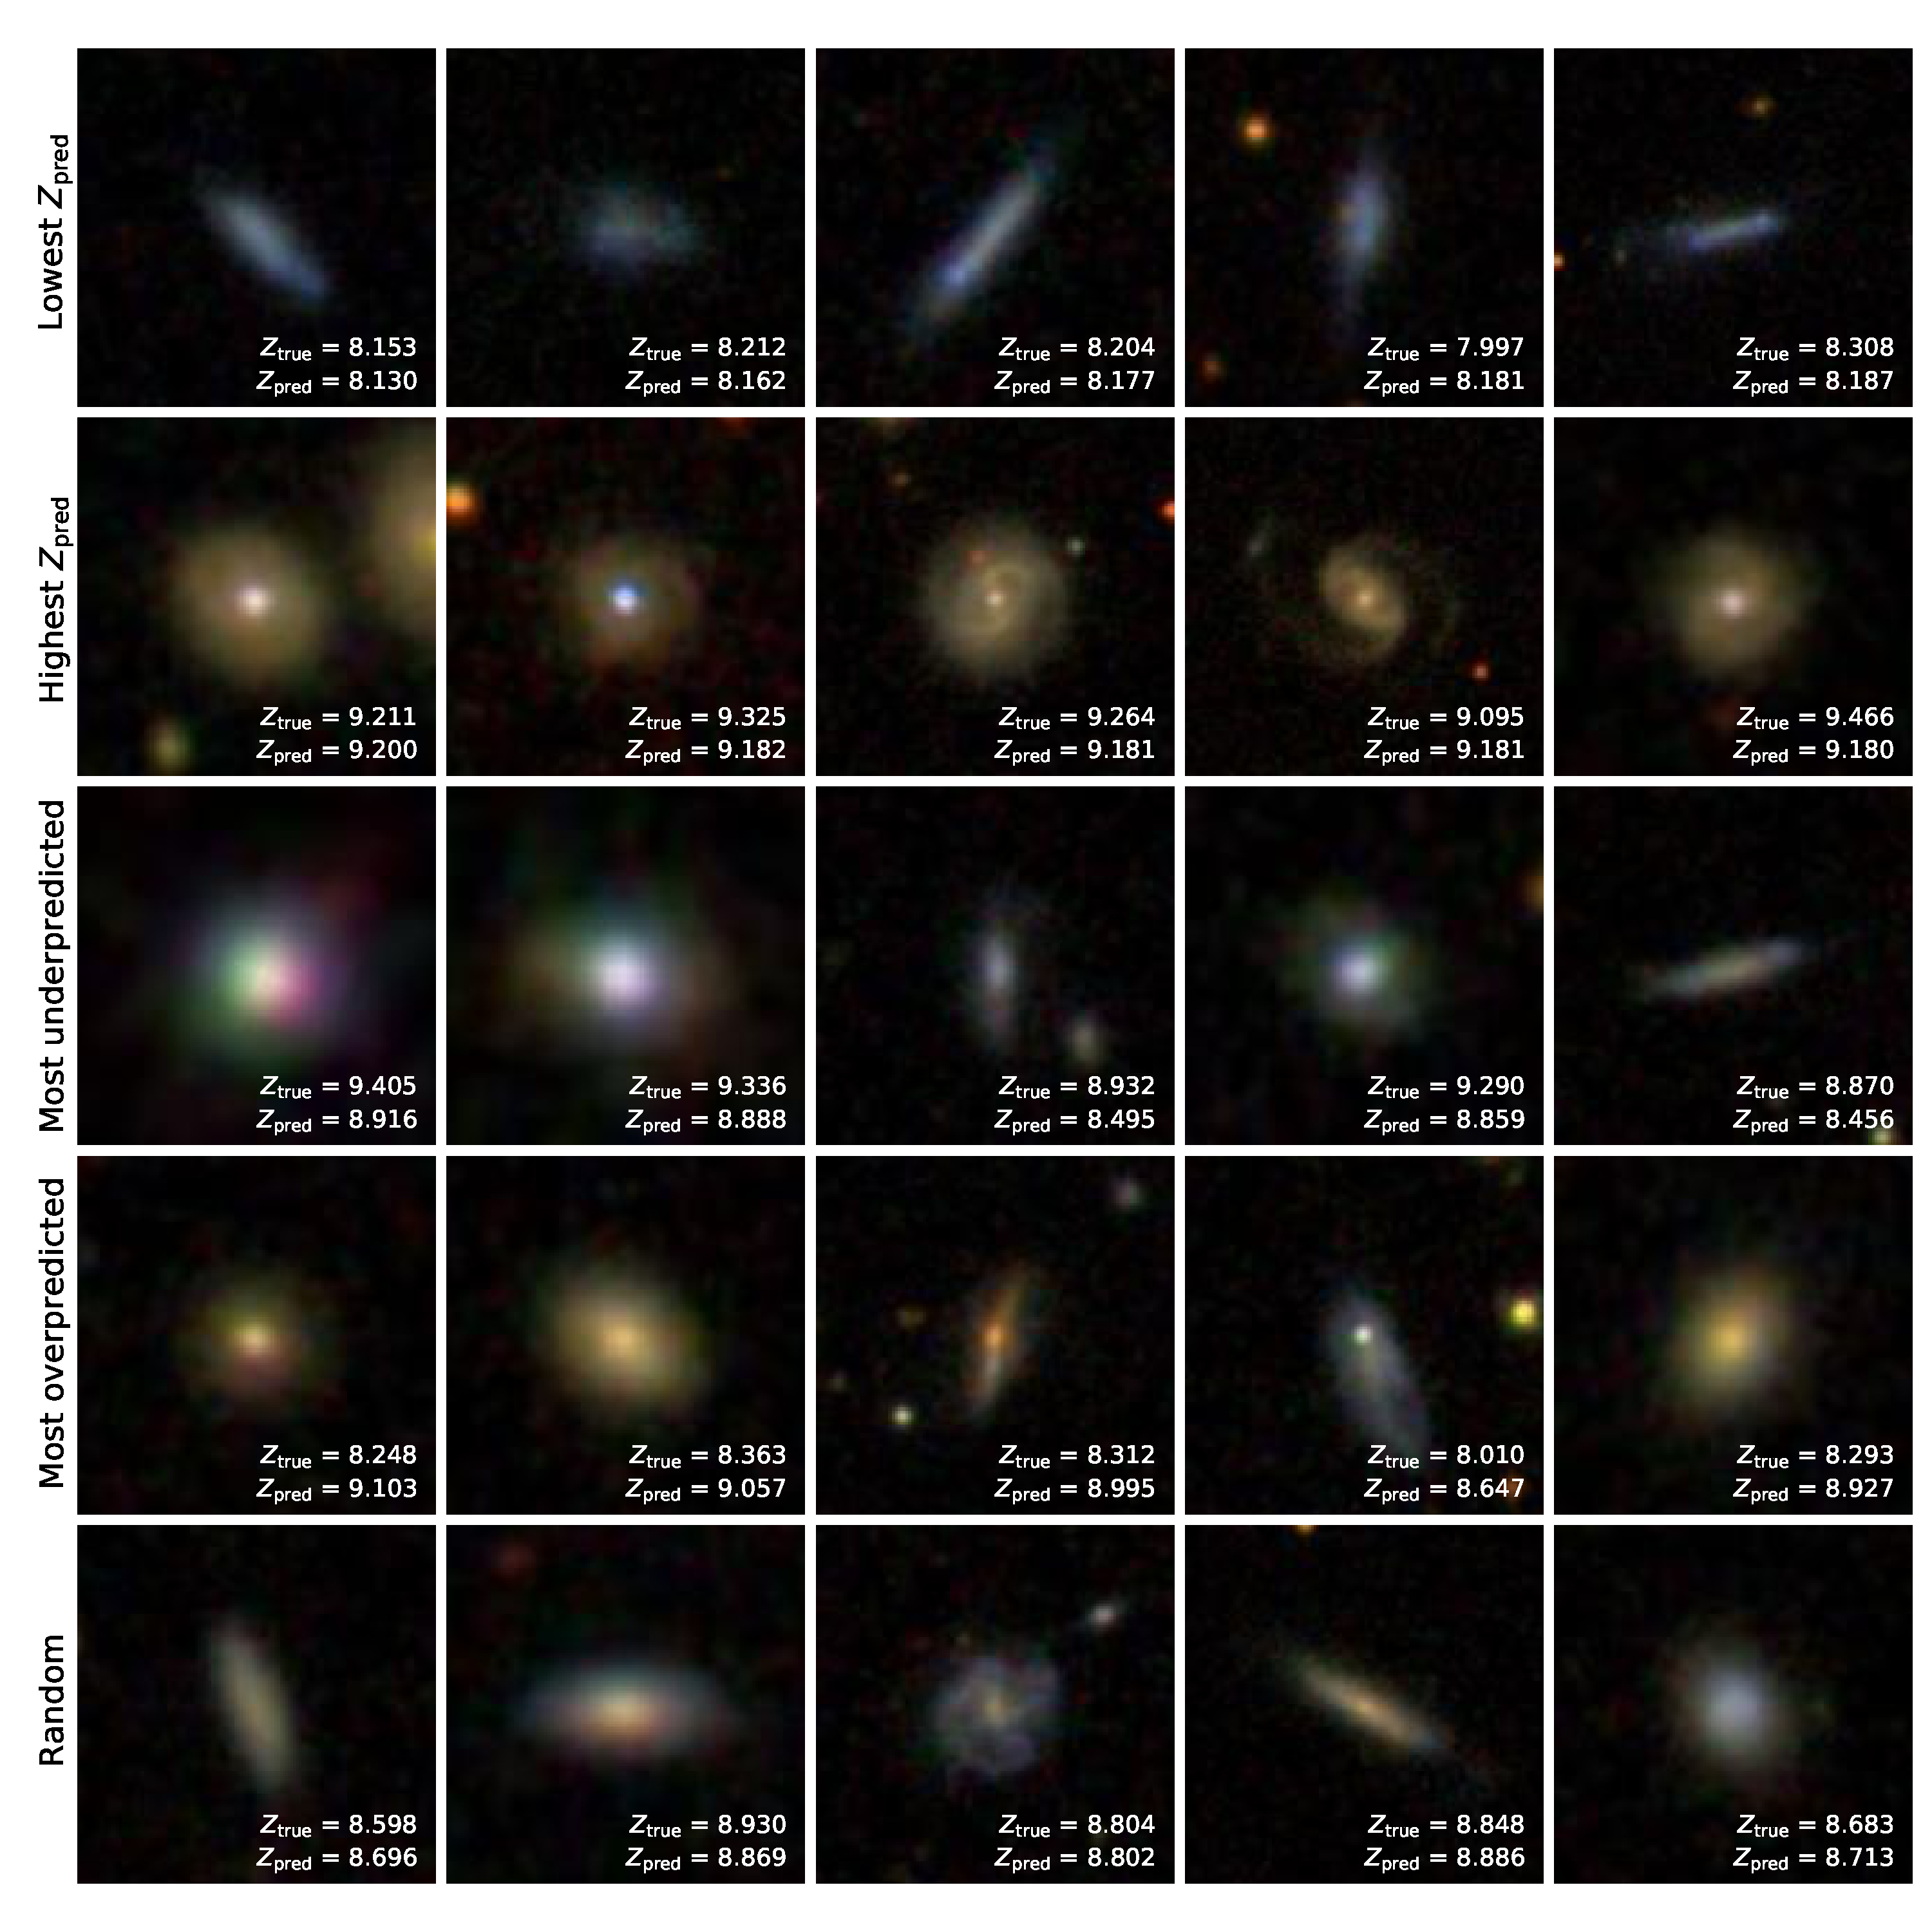
\includegraphics[width=0.9\textwidth]{01-prediction_examples.pdf}
	\caption{\label{fig:examples}
		SDSS imaging with predicted and true metallicities from the test data set. Five examples are shown from each of the following categories: (a) lowest predicted metallicity, (b) lowest true metallicity, (c) highest predicted metallicity, (d) highest true metallicity, (e) most under-predicted metallicity, (f) most over-predicted metallcity, and (g) a set of randomly selected galaxies.}
\end{figure*}

In Figure~\ref{fig:examples}, we show examples of $128 \times 128$ pixel \sdssi\sdssr\sdssg\ SDSS images that are evaluated by the CNN. Rows (a) and (b) depict the galaxies with lowest predicted and lowest true metallicities, respectively. The CNN has associated blue, edge-on disk galaxies with low metallicities, and is generally accurate in its predictions of low $Z_{\rm pred}$. In rows (c) and (d), we show the galaxies with highest predicted and highest true metallicities, respectively. Here we find that red galaxies containing prominent nuclei are predicted to be high in metallicity, and their predictions generally match $Z_{\rm true}$.

Galaxies predicted by our CNN to have high metallicities ($Z_{\rm pred} > 9.0$) tend to be characterized by high $Z_{\rm true}$, and the equivalent is true for low-metallicity galaxies. Inversely, galaxies with the highest (lowest) \textit{true} metallicities in the sample are also predicted to have high (low) metallicities. Note that inclined galaxies tend to be lower in metallicity whereas face-on galaxies appear to be higher in metallicity. \editorial{I can get the axis ratio if we want to do that test} \cite{Tremonti2004} explain this correlation by suggesting that the SDSS fiber aperture captures more column of a projected edge-on disk, allowing the metal-poor, gas-rich, and less-extincted outer regions to more easily be detected and depress the integrated $Z_{\rm true}$.

We will now consider examples of the most incorrectly predicted galaxies. In rows (e) and (f), we show instances in which the CNN predicted too low metallicity and too high metallicity, respectively. The two galaxies with lowest residuals $\Delta Z \equiv Z_{\rm pred} - Z_{\rm true}$ (\ie, most under-predicted metallicities) suffer from artifacts which cause nonphysical color gradients.\footnote{Note that both are labeled as quasars according to their SDSS DR14 spectra. \editorial{A. Baker mentioned that it is possible some of the incorrect predictions in Figure~1 may be due to the fact that the $R_{23}$ estimator is a double-valued function, and the particular branch chosen may cause incorrect estimation of $Z_{\rm true}$. Such an effect may be possible if, e.g., one of the oxygen lines is at low SNR and the uncertainties are large.}} Some of the other mistakes made by the CNN are similar to ones that would go against human intuition: blue, disky sources are generally thought of as lower in metallicity, and redder, more spheroidal objects tend to be higher in metallicity.

In the bottom row (g) of Figure~\ref{fig:examples}, we show five randomly selected galaxies. The random SDSS assortment consists of elliptical, spiral, and possibly even an interacting pair of galaxies. Residuals are low (below 0.15 dex), and we again find that the CNN predictions follow human visual intuition.

\subsection{Comparing Predicted and True Metallicities}
\begin{figure}
	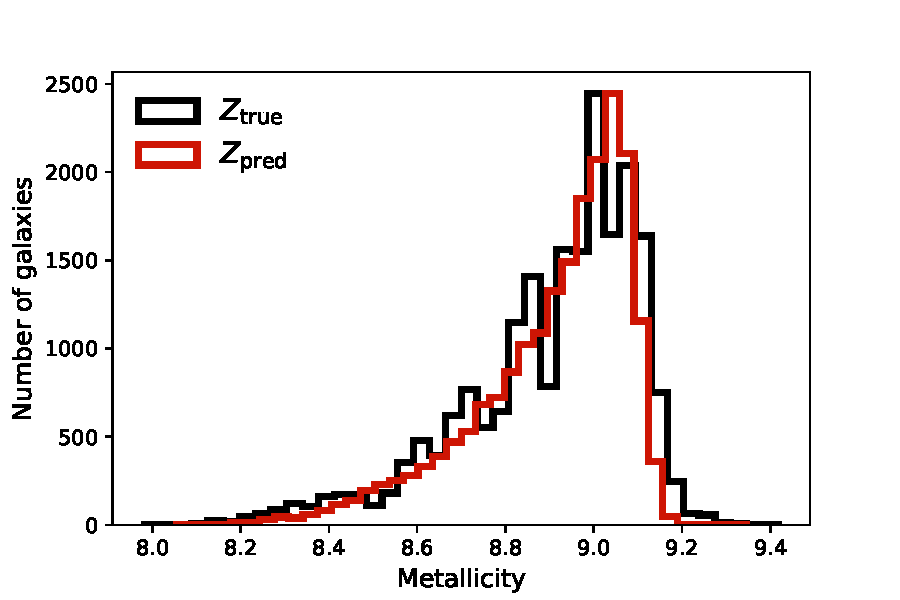
\includegraphics[width=\columnwidth]{03-Z_distribution.pdf}
	\caption{\label{fig:distributions}
		Distributions of the true (black) and predicted (red) galaxy metallicities. \editorial{A distribution of residuals is shown in the inset panel.} Note that the bin widths are different for each distribution. See text for details.}
\end{figure}

In Figure~\ref{fig:distributions}, we show the distributions of true and predicted metallicities as a black and red histogram respectively. The histogram bin sizes are chosen according to the \cite{Freedman1981} rule for each distribution. The discreet striping of the \cite{Tremonti2004} and \cite{Brinchmann2004} metallicity estimator appears in the $Z_{\rm true}$ distribution but does not manifest in our CNN predictions. This should increase the scatter in our distribution of residuals.

%Because the true metallicities are discreetly valued, we expect that our distribution of $\Delta Z$ will be heavy-tailed, since predicted values still be distributed smoothly over the peaks and troughs in the $Z_{\rm true}$ distribution. We also expect some outlier predictions at very negative or positive $\Delta Z$ for other reasons.

As we have described previously, the range of $Z_{\rm pred}$ is more limited than the range of $Z_{\rm true}$. Too narrow a domain in $Z_{\rm pred}$ will lead to systematic errors, as the CNN will end up never predicting very high or very low metallicities. Although the two distributions are qualitatively consistent with each other at low metallicities (\eg, $Z < 8.5$). \editorial{check numbers} However, the fraction of galaxies with high $Z_{\rm true} > 9.1$ ($2573/20466 = 12.6\%$) is more abundant than the fraction with high $Z_{\rm pred} > 9.1$ ($1174/20466 = 5.7\%$).
%However, $Z_{\rm true} > 9.1$ makes  of the test data set, whereas for only $1174/20466 = 5.7\%$ of predictions exceed $9.1$, so this discrepancy will lead to a shift toward negative residuals.

We find that the mode of the predicted metallicity distribution is higher than the mode of $Z_{\rm true}$. This result may be a consequence of the CNN overcompensating for its systematic under-prediction of metallicity for galaxies with $Z_{\rm true} > 9.1$. However, its effect on the entire distribution is small, and may be remedied simply by increasing the relative fraction of very high-$Z_{\rm true}$ objects. We find overall good agreement between the $Z_{\rm pred}$ and $Z_{\rm true}$ distributions. \editorial{t-test? quantify}

\subsection{Scatter in $Z_{\rm pred}$ and $Z_{\rm true}$}
\begin{figure}
	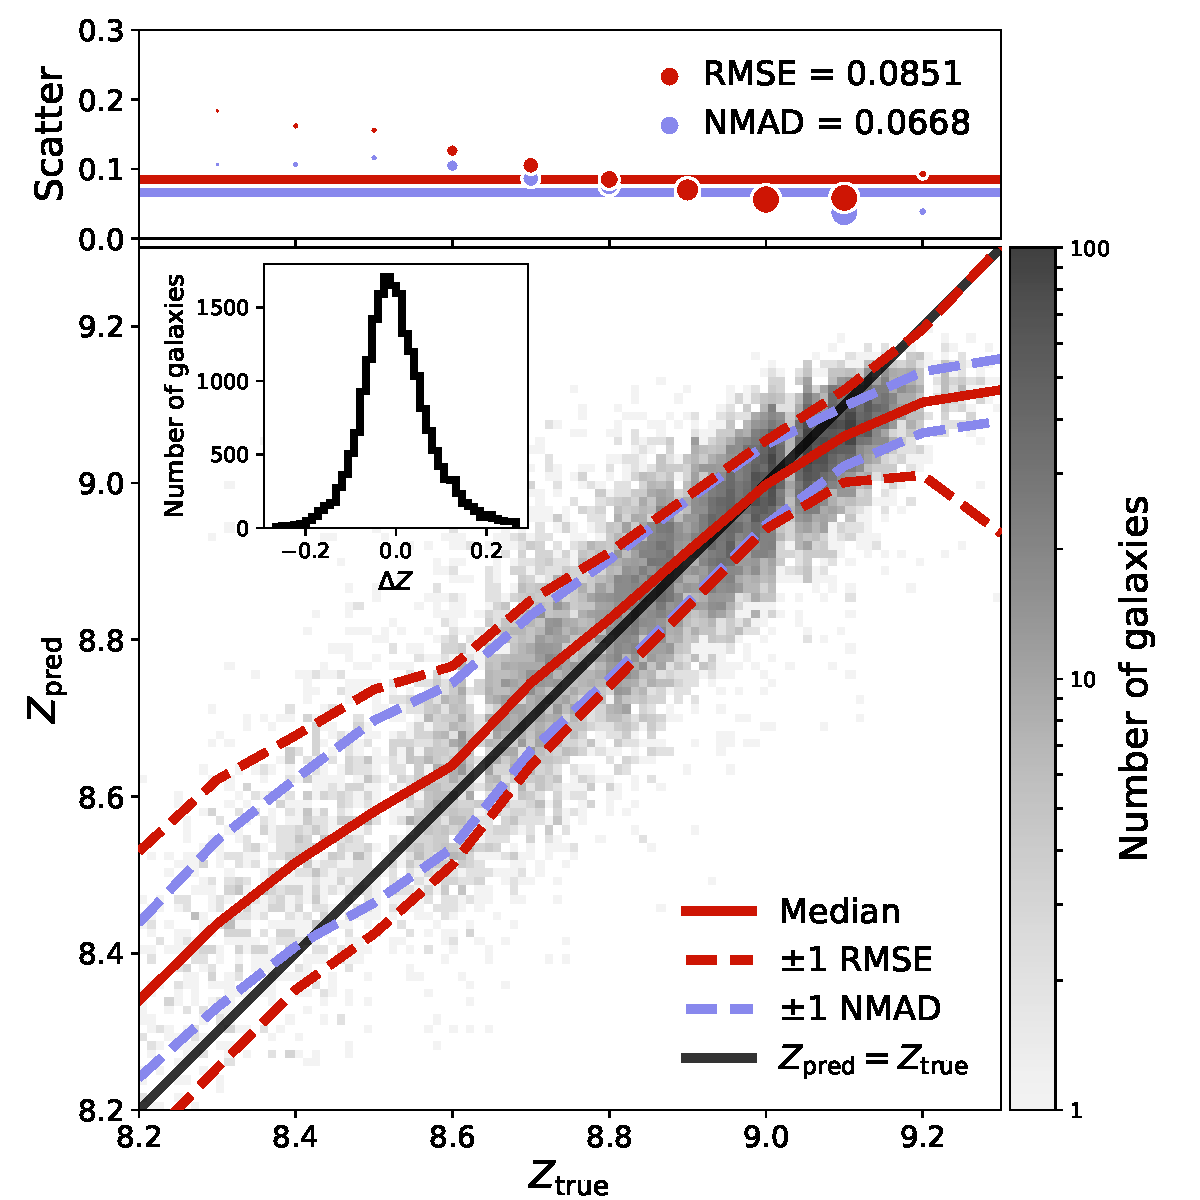
\includegraphics[width=\columnwidth]{02-prediction_summary.pdf}
	\caption{\label{fig:predicting-metallicity}
		Bivariate distribution of true galaxy metallicity ($Z_{\rm true}$) and CNN predictions ($Z_{\rm pred}$) are shown in the main panel. Overlaid are the median predicted metallicity, solid red line, RMSE scatter, dashed blue line, NMAD scatter, dashed orange line, in bins of $Z_{\rm true}$. The solid black line shows the one-to-one relation. In the upper panel, we again show the binned scatter, where the size of each marker is proportional to the number of galaxies in that bin. Each horizontal line corresponds to the average scatter over the entire test data set (and global value indicated in the upper panel legend).}
\end{figure}

In Figure~\ref{fig:predicting-metallicity}, we compare the distributions of $Z_{\rm true}$ and $Z_{\rm pred}$ using a two-dimensional histogram (shown in grayscale in the main, larger panel). We also show the median predictions varying with binned $Z_{\rm true}$ (solid red line), along with the scatter in RMSE (dashed blue) and NMAD (dashed orange), and also the one-to-one line (solid black). The running median agrees well with the one-to-one line, although at low metallicity we find that the CNN makes makes overpredictions.
%Thus, even though $Z_{\rm pred}$ and $Z_{\rm true}$ are in agreement at $Z < 8.5$ in Figure~\ref{fig:distributions}, we now find that the low-metallicity predictions are systematically too high.

A histogram of metallicity residuals is shown in the inset plot of the Figure~\ref{fig:predicting-metallicity} main panel. The $\Delta Z$ distribution is characterized by an approximately normal distribution with a heavy tail at large positive residuals; this heavy tail is likely due to the systematic over-prediction of low-$Z_{\rm true}$ galaxies.
%The median value of the distribution is $-0.006$, and a best-fit Gaussian function yields a centroid at $-0.009$.
There is also an overabundance of large negative $\Delta Z$ corresponding to under-predictions at high $Z_{\rm true}$, although this effect is smaller (despite appearing to be more significant in Figure~\ref{fig:distributions}).

We now turn our attention to the upper panel of Figure~\ref{fig:predicting-metallicity}, which shows how the scatter varies with spectroscopically derived metallicity. The RMSE scatter and outlier-insensitive NMAD are both shown. Marker sizes are proportional in area to the number of samples in each $Z_{\rm true}$ bin, and the horizontal lines are located at the average loss (RMSE or NMAD) for the full test data set.

Predictions appear to be both accurate and low in scatter for galaxies with $Z_{\rm true} \approx 9.0$, which is representative of a typical metallicity in the SDSS sample. Where the predictions are systematically incorrect, we find that the RMSE increases dramatically. However, the same is not true for the NMAD; at $Z_{\rm true} < 8.5$, it asymptotes to $\sim 0.10$, even though the running median is incorrect by approximately the same amount! This is because the NMAD determines the scatter about the \textit{median} and not $\Delta Z = 0$, and thus, this metric becomes somewhat unreliable when the binned samples do not have a median value close to zero. Fortunately, the global median of $\Delta Z$ is $-0.006$, or less than 10\% of the RMSE, and thus the global NMAD $= 0.0668$ is representative of the outlier-insensitive scatter for the entire test data set.

This effect partly explains why the global NMAD (0.0668) is higher than the weighted average of the binned NMAD ($\sim 0.05$).Also, each binned NMAD is computed using its local scatter, such that the outlier rejection criterion varies with $Z_{\rm true}$. To illustrate this effect with an example: $\Delta Z \approx 0.2$ would be treated as an $3~\sigma$ outlier at $Z_{\rm true} = 9.0$, where the CNN is generally accurate, but the same residual would not be rejected as an outlier using NMAD for $Z_{\rm true} = 8.5$.
Since the binned average NMAD depends on choice of bin size, we do not include those results in our analysis and only focus on the global NMAD.

\subsection{Resolution effects} \label{sec:resolution}
%Note by the way that our CNN trained on color images is able to predict better than by using only photometry (via random forest) and morphology ($r$-band CNN) independently.
%Perhaps this is due to the fact that morphology is correlated with stellar population age or something else.
%Color tells us the fundamental plane of SFR-$M_*$-metallicity but is biased by age and dust.

\begin{figure}
	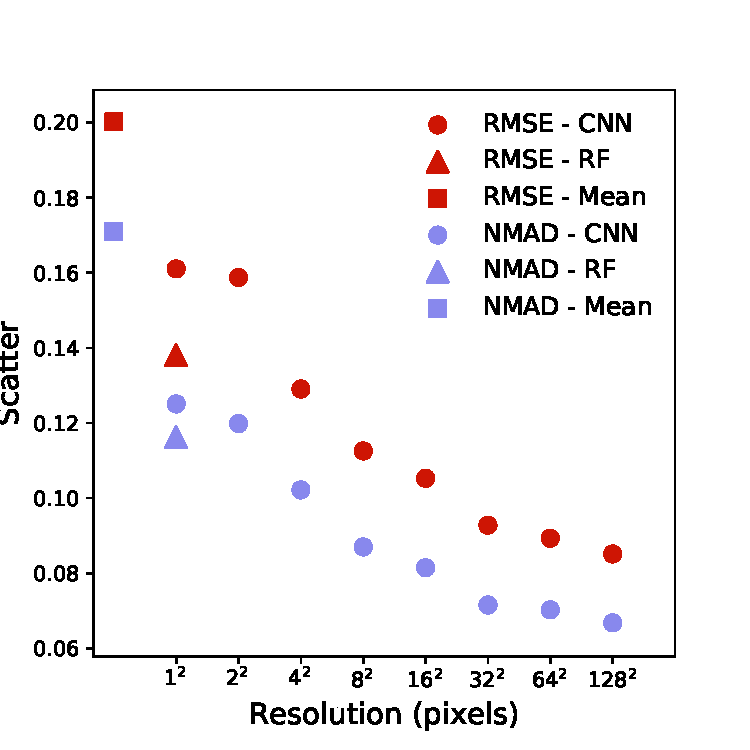
\includegraphics[width=\columnwidth]{04-resolution.pdf}
	\caption{\label{fig:resolution}
		The effects of image resolution on CNN performance. Blue and orange circular markers indicate scatter in the residual distribution ($\Delta Z$) measured using RMSE and NMAD, respectively. (Each point is analogous to the horizontal lines shown in Figure~\ref{fig:predicting-metallicity}.) We also show predictions from a random forest algorithm as stars-shaped markers, and constant $\langle Z_{\rm true}\rangle$ predictions as square markers.}
\end{figure}

Because our methodology is so computationally light, we can run the same CNN training and test procedure on images scaled to different sizes in order to consider the effects of image resolution. Our initial results use SDSS $15\arcsec \times 15 \arcsec$ cutouts resized to $128\times 128$ pixels, and we now downsample the same images to $64\times 64$, $32 \times 32$, $\cdots$, $2\times 2$, and even $1\times 1$ pixels via re-binning. All images retain their three channels, so the smallest $1 \times 1$ image is effectively the pixels in each of the \sdssi\sdssr\sdssg-bands averaged together with the background and possible neighboring sources.

In Figure~\ref{fig:resolution}, we show the effects of image resolution by measuring the global scatter in $\Delta Z$ using the RMSE and NMAD metrics (shown in blue and orange circular markers, respectively). Also shown is the scatter in $\Delta Z$ if we always predict the mean value of $Z_{\rm true}$ over the data set (shown using a square marker). This constant prediction is effectively the worst-possible scatter, and the \cite{Tremonti2004} systematic uncertainty in $Z_{\rm true}$ of $\sim 0.03$~dex is the best-possible scatter. We find that both RMSE and NMAD decrease with increasing resolution, as expected if morphology or color gradients are instrumental to predicting metallicity.
%In nearly all cases, we find that the NMAD is lower than the RMSE by a factor of $\sim 3/4$.

There appears to be little improvement in scatter going from $1 \times 1$ to $2\times 2$ pixel images. $1\times 1$ three-color images contain similar information to three photometric data points (although because of the included background and neighboring pixels, it is less useful than photometry), which can be used to perform a crude spectral energy distribution (SED) fit.
%The color information is useful enough to create an approximate color-magnitude diagram, and each galaxy's position in this parameter space correlates with $Z_{\rm true}$.
Therefore it unsurprising that the $1 \times 1$ CNN predictions perform so much better than the baseline mean prediction. A $2 \times 2$ three-color image contains four times as many pixels as a $1\times 1$ image, but because the object is centered between all four pixels, this information is still averaged among all available pixels. Therefore, the scatter does not improve appreciably between $1 \times 1$ and $2 \times 2$ resolutions.\footnote{There is extra information in the $2\times 2$ pixel images in non-circularly symmetric cases. For an inclined disk, it is possible to roughly determine the orientation in the sky plane, but this information is not very useful. In the case of a major merger or interacting companion, the $2\times 2$ images may be more powerful than $1 \times 1$ images.}

The scatter is a strong function of resolution as the images are resolved from $2 \times 2$ to about $32 \times 32$. With further increasing resolution, improvement is still evident, although the scaling with scatter is noticeably weaker. Because the angular size of each image cutout stays the same, the pixel scale changes from $0\farcs469$/pix for $32 \times 32$ images, to $0\farcs234$/pix for $64 \times 64$ images, to $0\farcs117$/pix for $128 \times 128$ images. The native SDSS pixel resolution is $0\farcs396$/pix, such that the $64 \times 64$ and $128 \times 128$ resolutions result in the oversampling of each image! Thus, the plateauing of scatter with resolution is expected for images larger than $32 \times 32$. It is worth noting, however, that the CNN attempts to learn filters which depend on the size of the input image, and that smaller images may result in the CNN training filters that are too low in resolution to be completely effective for prediction. Therefore, it is also not surprising that the CNN makes incremental gains for images with increasing resolution beyond $32 \times 32$ pixels.

\subsection{Random Forest Predictions for Metallicity}
We also construct a random forest (RF) of decision trees in order to predict metallicity using the implementation from \texttt{scikit-learn} \citep{Pedregosa2012}. Hyperparameters are selected according to the optimal RF trained by \cite{Acquaviva2016}. We use exactly the same data labels (\ie, galaxies) to train/validate or test the RF as we have used for training and testing the CNN, so that our measurements of scatter can be directly compared. However, we have used the $gri$ three-band photometry data (given in magnitudes) to train and predict metallicity. Since each galaxy only has three pieces of photometric information, it can be compared to the $1 \times 1$ three-band ``images'' processed by our CNN.

We note that the RF outperforms the CNN results using $1\times 1$ and $2 \times 2$ images.
This result is unsurprising because the RF is supplied aperture-corrected photometry, whereas the CNN is provided $1 \times 1 $ \sdssi\sdssr\sdssg ``images'' whose features have been averaged with their backgrounds. $2 \times 2$ images are only marginally more informative. When the resolution is further increased to $4 \times 4$ images, then the CNN can begin to learn rough morphological features and color gradients, which is already enough to surpass the performance (measured by both RMSE and NMAD) of the RF.
\editorial{This result suggests that the CNN is able to learn a nontrivial representation of gas-phase metallicity based on morphology, even with extremely low-quality data.}

\subsection{Comparisons to Previous Works}\label{sec:previous work}
CNNs have been used for a wide variety of classification tasks in extragalactic astronomy, including morphological classification \citeeg{Dieleman2015, Huertas-Company2015, 2017MNRAS.464.4420S}, distinguishing between compact and extended objects \citep{Kim2017}, selecting observational samples of rare objects based on simulations \citep{Huertas-Company2018, Lanusse2017}, and visualizing high-level morphological galaxy features \citep{Dai2018}. These works seek to improve classification of objects into a discreet number of classes, \ie, visual morphologies. Our paper uses CNNs to tackle the different problem of regression, \ie, predict values from a continuous distribution.
% Ellison group? 2016MNRAS.455..370E, 2017MNRAS.464.3796T, 2016MNRAS.457.2086T
% also 2018MNRAS.476.5516B?

Examples of regressing stellar properties in the astronomical ML literature \citeeg{2000A&A...357..197B, Fabbro2018}, they train on synthetic stellar spectra and test on real data. Their predicted measurements of stellar properties, \eg, stellar effective temperature, surface gravity, or elemental abundance, are able to be derived from the available training data set. Our work is novel because we predict metallicity, a spectroscopically determined galaxy property, using only three-color images. Said another way, it is not necessarily the case that $Z$ can be predicted from our training data. However, we find that galaxy morphology supplements color information that is useful for predicting metallicity.

A similar study to this work is that of \cite{Acquaviva2016}. The authors use a variety of machine learning methods including RFs, extremely random trees (ERTs), boosted decision trees (AdaBoost), and support vector machines (SVMs) in order to estimate galaxy metallicity. The \cite{Acquaviva2016} data set consisted of a $z \sim 0.1$ sample (with $\sim 25,000$ objects) and a $z \sim 0.2$ sample (with $\sim 3,000$ objects), each of which had five-band SDSS photometry ($ugriz$) available as training data. These samples are sparsely populated at low metallicities, and they contain a smaller fraction of objects with $Z_{\rm true} < 8.5$ than our sample, but are otherwise similarly distributed in $Z_{\rm true}$ to ours. \editorial{The estimates of Z come from the same place, so we are really using a similar catalog. Why are there so much fewer objects in her catalog?}

We will first compare RF results, since this technique is common to both of our analyses, and reveals important differences in our training data. Because outliers are defined differently in both works, we will use the RMSE metric to compare scatter between the two. \cite{Acquaviva2016} obtained RMSE of 0.081 and 0.093 dex when using RFs on the five-band photometry. Using the same RF approach on a larger sample, while working with only \textit{three} bands of photometric information, we find RMSE $= 0.130$ dex. Our scatter is larger than the value reported by \cite{Acquaviva2016} by a factor of $\sim 150\%$. This result may partly be explained by the fact that their $Z_{\rm true}$ distribution is narrower than for our \editorial{training?} data set, or the fact that our data set spans a broader range in galaxy redshift; however, some of this advantage is offset by our larger sample size.

Ultimately, it appears the extra \sdssu and \sdssz bands supply machine learning algorithms with valuable information for predicting metallicity. % and allows for better estimation of metallicity.
% rfs using the added photometry data output $Z_{\rm pred}$ with significantly lower scatter than our using only $gri$ bands.
Indeed, the \sdssu\ and \sdssz-bands convey information about the galaxy's star formation rate (SFR) and stellar mass (\mstar) \editorial{can we find a citation for this?}. For this reason, it is possible that the RF trained on five-band photometry can estimate $Z_{\rm true}$ down to the limit of the FMR, which has very small scatter ($\sim 0.05$ dex) at given \editorial{fixed?} $M_{\star}$ \textit{and} SFR. The \sdssg, \sdssr, and \sdssi-bands are rather insensitive to the SFR, but can still provide some information about the stellar mass, and so its results are more linked to the MZR rather than the FMR.

Regardless of these limitations, our CNN is able to estimate metallicity with $\Delta Z = 0.085$ dex, which is comparable to the scatter in residuals using the best algorithms from \cite{Acquaviva2016}. There is evidence that the morphological information provided by using images rather than photometric data is helping the CNN perform so well: (1) the RMSE scatter decreases with increasing image resolution, and (2) it identifies edge-on galaxies as lower-$Z_{\rm true}$ and face-on galaxies as higher-$Z_{\rm pred}$ (consistent with observational bias). Gradients in color, or identification of mergers \citeeg{Ackermann2018} may also be helpful for predicting metallicity.

\editorial{really like this section}

\section{The mass-metallicity relation} \label{sec:MZR}
The MZR describes the tight correlation between galaxy stellar mass and nebular metallicity. Scatter in this correlation is approximately $\sigma \approx 0.10$ dex in $Z_{\rm true}$ over the stellar mass range $8.5 < \log (\mstar / \msol) < 11.5$ \citep{Tremonti2004}, where $\sigma$ is the standard deviation of the metallicity and is equivalent to the RMSE for a normal distribution. The MZR can be characterized empirically using a polynomial fit:
\begin{equation}\label{eq:mzr}
Z = -1.492 + 1.847 \log (\mstar / \msol) - 0.08026 \left [\log(\mstar / \msol)\right ]^2.
\end{equation}

The physical interpretation of the MZR is that a galaxy's \editorial{stellar?} mass strongly correlations with its chemical enrichment. Proposed explanations of this relationship's origin include metal loss through blowout \citep[e.g.,][]{2002ApJ...581.1019G,Tremonti2004} inflow of pristine gas, or a combination of the two \citep[][]{2013ApJ...772..119L}; however, see also \cite{2013A&A...554A..58S}. Although the exact physical process responsible for the low ($0.10$ dex) scatter in the MZR is not known, its link to SFR via the FMR is clear, as star formation leads to both metal enrichment of the interstellar medium and stellar mass assembly.

The FMR connects the instantaneous ($\sim 10$ Myr) SFR with the gas-phase metallicity \citep[$\sim 1$~Gyr timescales; see, e.g.,][]{2011ApJ...734...48L} and \mstar\ (\ie, the $\sim 13$~Gyr integrated SFR). Our CNN is better suited for predicting \mstar\ rather than SFR, using the $gri$ bands, which can only weakly probe the blue light from young, massive stars. Therefore, we expect the scatter in CNN predictions to be limited by the MZR (with scatter $\sigma \sim 0.10$ dex) rather than the FMR ($\sigma \sim 0.05$~dex). It is possible that galaxy color and morphology, in tandem with CNN-predicted stellar mass, can be used to roughly estimate the SFR, but in this paper we will focus on only the MZR.

%Given the low scatter in metallicity residuals (predicted $-$ true), we consider if the CNN is able to accurately predict stellar mass, and then leverage the mass-metallicity relation (MMR; Tremonti et al. 2004) to infer metallicity.
%Alternatively, if SFR and $M_*$ are learned, then the fundamental metallicity relation (FMR; Mannucci et al. 2010, Lara-Lopez et al. 2010) may explain low residuals.

\subsection{Predicting Stellar Mass}

\begin{figure*}
	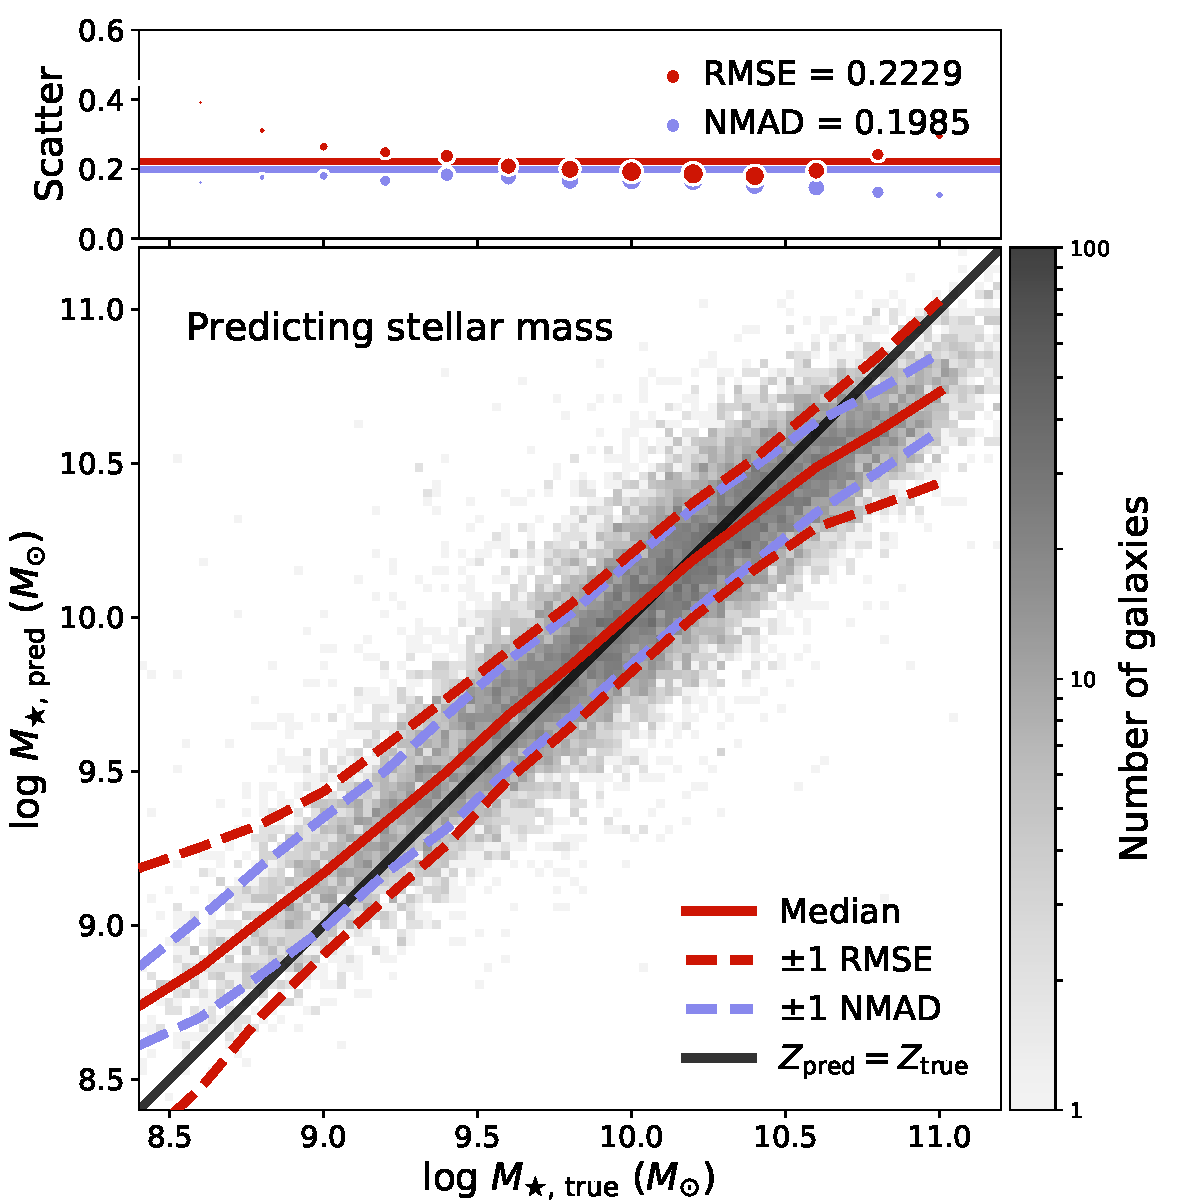
\includegraphics[width=\columnwidth]{05-a-prediction_mass.pdf}
	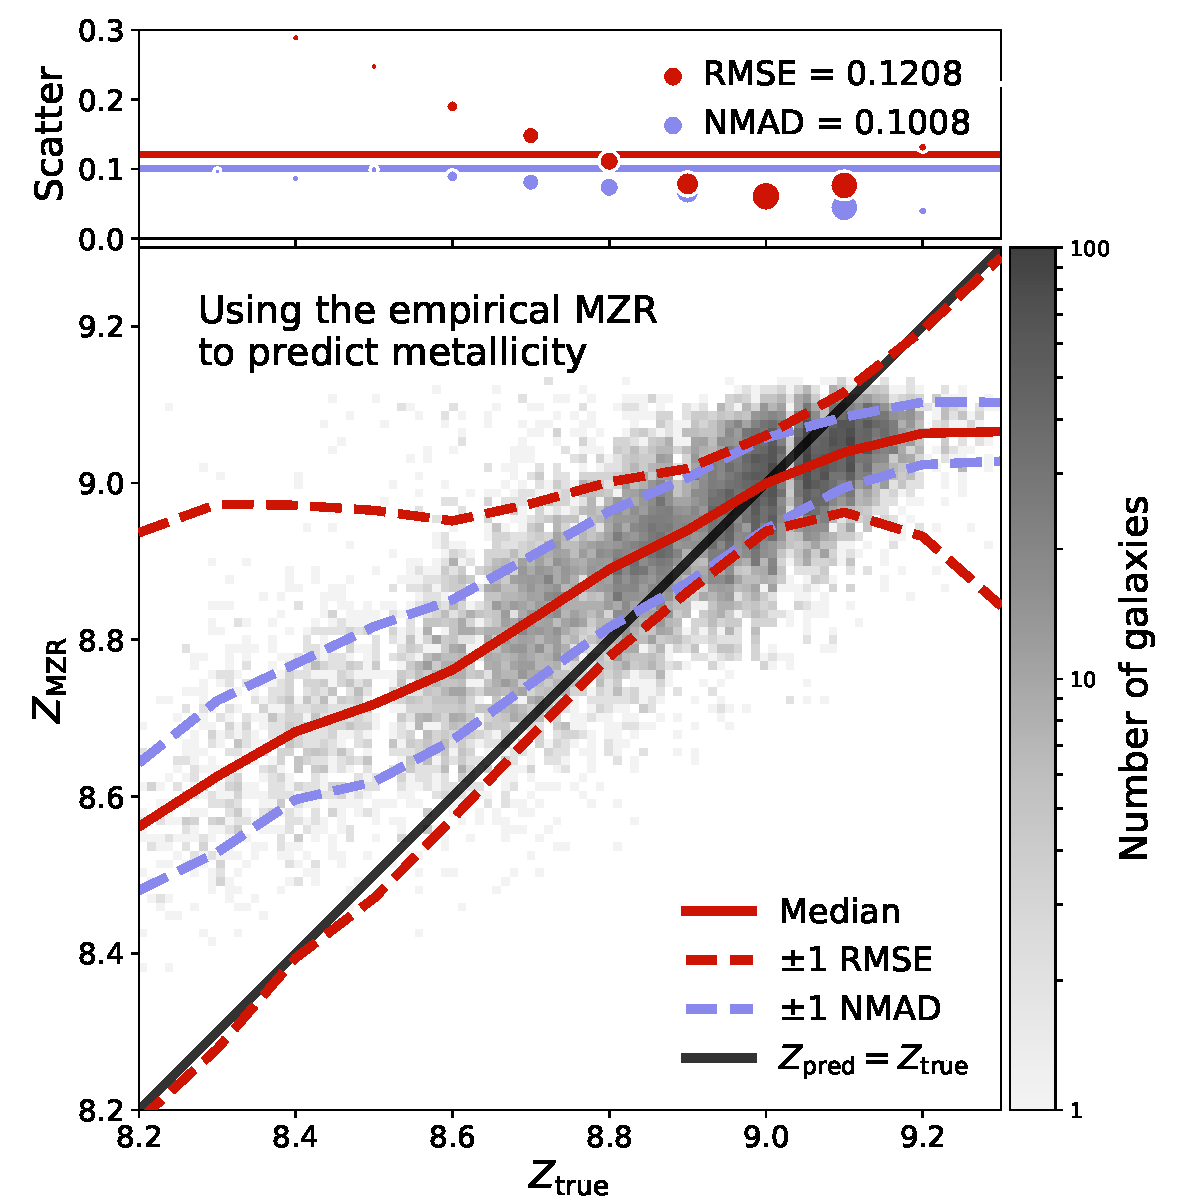
\includegraphics[width=\columnwidth]{05-b-prediction_mzr.pdf}
	\caption{\label{fig:mass-metallicity}
		In the left panel, we show the CNN predicted galaxy stellar mass against true stellar mass. Colors and marker or line styles are the same as in Figure~\ref{fig:predicting-metallicity}. In the right panel, we compare the predicted stellar mass converted to metallicity, assuming the \cite{Tremonti2004} MZR, with the true metallicity.}
\end{figure*}

Since galaxy stellar mass is known to correlate so strongly with metallicity, and is easier to predict (than, \eg, SFR) from \sdssi\sdssr\sdssg\ imaging, we consider the possibility that the CNN is simply predicting $M_{\star,\rm pred}$ accurately and then learning the simple polynomial transformation in order to predict metallicity. We can simulate this method by training the CNN on $M_{\star, \rm true}$ and then converting the stellar mass predictions to metallicities using Equation~\ref{eq:mzr}.

We re-run the CNN methodology to train and predict $M_{\star}$ using the 142,145 galaxies out of the original 142,186 that have available stellar mass measurements. These results are shown in the left panel of Figure~\ref{fig:mass-metallicity}. From the same subsample as before (minus three which do not have \mstar), we verify that $M_{\rm \star, true}$ median agrees with the median of $M_{\rm \star, true}$ for values between $9.0 \lesssim \log \mstar /\msol \lesssim 10.5$. The RMSE scatter in the \mstar residuals is $\sim 0.22$ dex, and the NMAD is $\sim 0.20$ dex. The slope of the empirical MZR at $\log (\mstar / \msol) \sim 10$ is (0.4 dex in $Z$)/(1.0 dex in \mstar), implying that the CNN might be able to leverage the MZR and predict metallicity to $\sim 0.08$ dex (plus any intrinsic scatter in the MZR, in quadrature).
%Given our CNN's ability to accurately predict $M_{\star}$, coupled with the inability of SDSS images to inform it about nebular regions or spectral lines, is it possible that the CNN's unexpectedly strong performance in predicting metallicity comes through the MZR?

%One option is that the CNN learned to predict $M_{\star}$ followed by the polynomial MZR transformation (Equation~\ref{eq:mzr}).
%We can simulate predicting metallicity this way by outputting $M_{\rm \star, pred}$, and then passing those predictions through the empirical MZR (which we will call $Z_{\rm MZR}$).

We use Equation~\ref{eq:mzr} and $M_{\star,\rm pred}$ to predict metallicity, which we call $Z_{\rm MZR}$.
In the right panel of Figure~\ref{fig:mass-metallicity}, we compare $Z_{\rm MZR}$ against $Z_{\rm true}$.
The scatter in residuals $Z_{\rm MZR} - Z_{\rm true}$ is $0.12$ dex, which is significantly higher than the $0.085$ dex scatter reported in Section~\ref{sec:results}.
%Intriguingly, however, the scatter is slightly lower than the $0.13{\rm ~ dex} \approx \sqrt{\rm (0.10~dex)^2 + (0.08~dex)^2}$ expected from independently adding the MZR scatter and $M_{\rm \star}$ prediction scatter in quadrature.

\editorial{This evidence suggests that the CNN has learned to determine metallicity in a more powerful way than by simply predicting $M_{\rm \star,pred}$ and then applying a polynomial conversion.}

\editorial{I think I am ok saying that. We shouldn't be afraid to be bold.}

\subsection{Lowering the scatter in the MZR}
\begin{figure}
	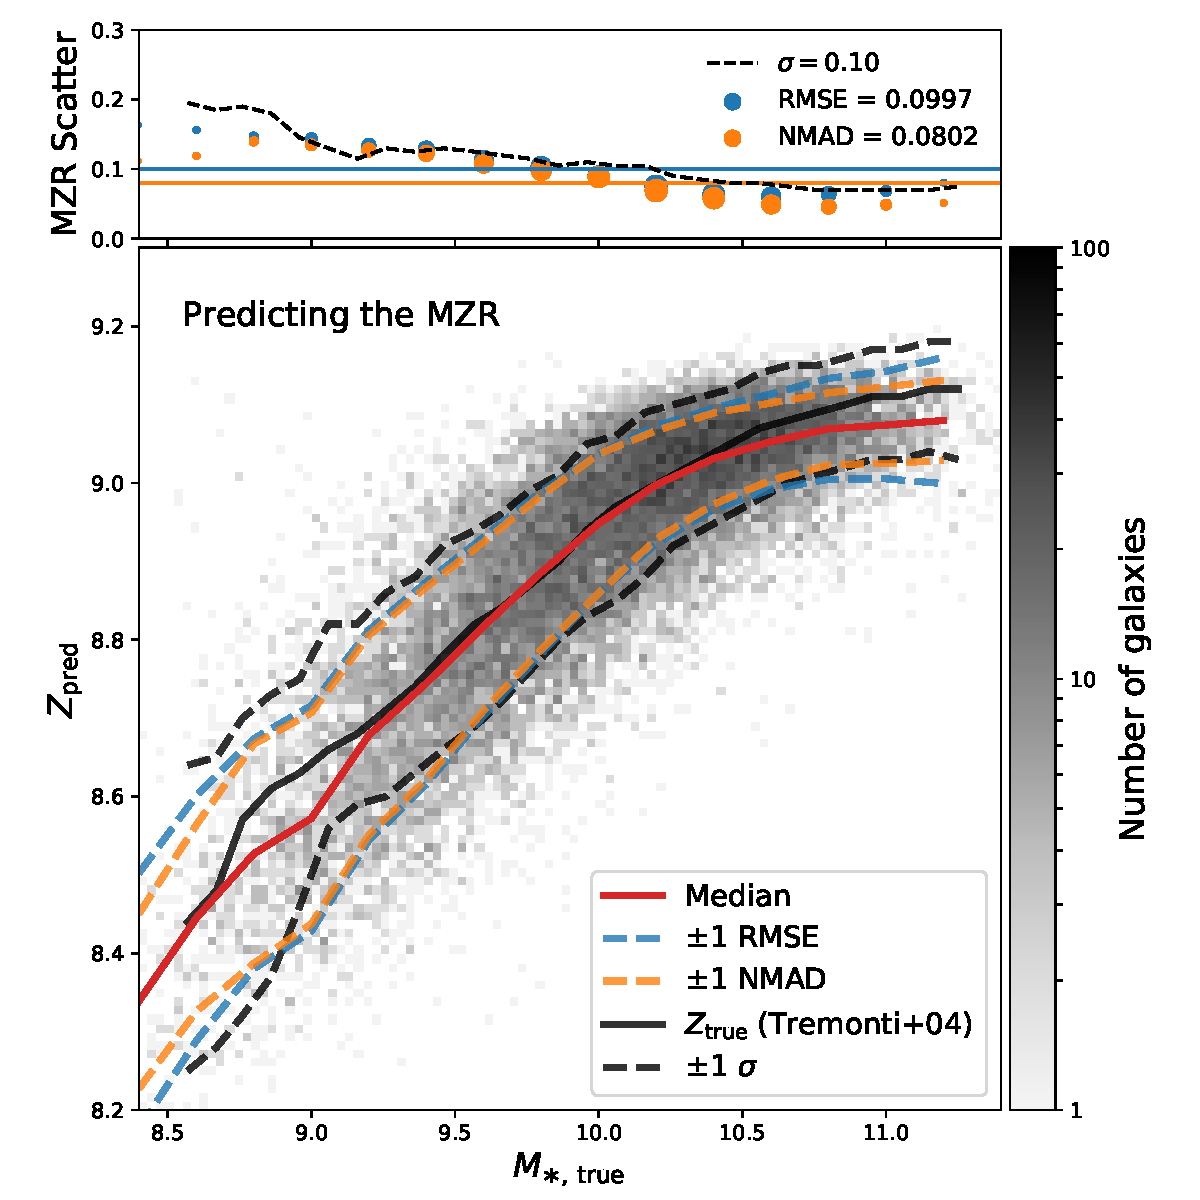
\includegraphics[width=\columnwidth]{05-mzr.pdf}
	\caption{\label{fig:mzr}
		In the main panel, the predicted MZR comparing true \mstar against CNN predicted $Z_{\rm pred}$ is shown in grayscale. The running median (solid red) and scatter (dashed blue and orange) are shown in 0.2 dex mass bins. For comparison, we also show the \citet{Tremonti2004} observed median and scatter binned by 0.1 dex in mass (solid and dashed black lines, respectively). In the top panel, we show the scatter in the predicted and empirical MZR. The standard deviation of the scatter in the MZR is shown as a dashed black line, while the blue and orange circles show the RMSE and NMAD, respectively, in bins of true \mstar. Marker sizes are proportional to the number of galaxies in each stellar mass bin. Global scatter in the CNN-predicted MZR appears to be comparable or even lower than scatter from the true MZR.}
\end{figure}

The RMSE $= 0.085$ dex difference between the true and CNN-predicted metallicities can be interpreted in one of two ways: (1) the CNN is inaccurate, and $Z_{\rm pred}$ deviates randomly from $Z_{\rm true}$, or (2) the CNN is labeling $Z_{\rm pred}$ according to some other hidden variable, and $\Delta Z$ represents a non-random shift in predictions based on this variable. If the first scenario is true, then we would expect the random residuals to increase the scatter of known correlations such as the MZR. If the second is true, then we would expect the tightness of such known correlations to remain unchanged.

In Figure~\ref{fig:mzr}, we show true stellar mass ($M_{\star, \rm true}$) against CNN-predicted metallicity. For comparison, we also overlay the \cite{Tremonti2004} MZR and its scatter ($\sigma = 0.10$ dex). The empirical median relation (solid black) matches our predicted MZR median (solid red), and the lines marking observed scatter (dashed black) appear to match observed scatter as well (dashed blue and orange). Over the range $9.5 \leq \log (M_{\star, \rm true}/\msol) \leq 10.5$, the RMSE scatter in $Z_{\rm pred}$ (dashed blue) appears to be even tighter than the observed $\pm 1-\sigma$ (dashed black). The same is true for the NMAD, which is even lower over the same interval.

In the upper panel of Figure~\ref{fig:mzr}, we present the scatter in both predicted and \cite{Tremonti2004} MZR binned by mass. We confirm that the CNN predicts a MZR that is at most equal (and possibly smaller) in scatter than one constructed using the true metallicity. The stellar mass bins for which the predicted RMSE is lower than measured $\sigma$ are the ones which contain the most training examples. \editorial{feel like this sentence is missing words} Thus, it may be possible that if our data set was augmented to include additional low- and high-$M_{\rm \star,true}$ galaxies, then the predicted RMSE (and NMAD) may be even lower.

The fact that a CNN trained on only \sdssi\sdssr\sdssg\ imaging is able to predict metallicity accurately enough to reproduce the MZR in terms of median and scatter is not trivial. The error budget is very small: $\sigma = 0.10$ dex affords only, \eg, 0.05 dex of scatter when SFR is a controlled parameter plus a 0.03 dex systematic scatter in $Z_{\rm true}$ measurements, leaving only $\sim 0.08$ dex remaining for CNN systematics.

This is somewhat compatible with our result of RMSE($\Delta Z$) $= 0.085$. However, this cannot be correct since it assumes that the CNN is recovering the FMR perfectly -- and as we have discussed before, it is highly unlikely that the CNN is sensitive to the SFR and therefore cannot probe the MZR at individual values of the SFR. The error budget for the MZR is already exceeded, too, as we have found RMSE $= 0.10$ dex for both the $Z_{\rm pred}-M_{\star,\rm true}$ relation and the empirical MZR ($Z_{\rm true}-M_{\star,\rm true}$) without accounting for the fact that $Z_{\rm pred}$ and $Z_{\rm true}$ differ by RMSE $= 0.085$ dex!

We thus find more evidence that the CNN has learned something from the SDSS \sdssi\sdssr\sdssg imaging that is different from, but at least as powerful as, the MZR. One way that this is possible is if the CNN can measure some version of metallicity that is more fundamentally linked to the stellar mass, rather than $Z_{\rm pred}$ as derived from oxygen spectral lines. Another possibility is that the MZR is a projection of a correlation between stellar mass, metallicity, and a third parameter, perhaps one that is morphological in nature. If this is the case, then the \cite{Tremonti2004} MZR represents a relationship that is randomly distributed in the yet unknown third parameter, while our CNN would be able to stratify the MZR according to this parameter (much like how the FMR does so with the SFR). We are unfortunately not able to identify any hidden parameter using the current CNN methodology, but we plan to explore this topic in a future work.

\editorial{this is good stuff}

%Note that we did not plot $M_{\rm \star,~pred}$ because any possible covariance in the predicted metallicity and stellar mass would make such a MZR appear to be more correlated than it truly is.


%If there existed a fourth parameter, perhaps morphological in nature, then the marginalized MMR or FMR over particular values of this fourth parameter should be an even tighter relationship.
%Such a result would be analogous to how the MMR at any given star formation rate (SFR) has smaller scatter than over all SFRs.
%
%We find that the MMR constructed using SDSS-measured metallicity (via $R_{23}$) and the MMR constructed using CNN-predicted metallicity (from \textit{gri} imaging) are quantitatively different.
%In both cases we have used the GalSpecExtra catalog for stellar masses.
%The MMR using CNN metallicity has smaller scatter, where the weighted average ratio of scatter is NMAD(CNN)/NMAD(SDSS)~$= 0.821 \pm 0.077$.


%We also produced plots of the MMR using SDSS- and CNN-predicted masses, and SDSS metallicity from the GalSpecExtra catalog.
%Here the scatter in metallicity at given mass is again lower when using CNN predictions than for SDSS measurements.
%The scatter is smaller by a factor NMAD(CNN)/NMAD(SDSS)~ $= 0.811 \pm 0.057$.
%
%It is possible that the metallicity depends on some morphological component in addition to the emission lines informing the spectroscopic measurement.
%However, we believe that the qualitatively accurate MMR is actually artifact of the CNN's limitations rather than its strengths.
%Instead of finding a more fundamental representation of metallicity, the CNN likely detects the stellar mass.
%In the case of using our CNN to predict metallicity, the slope of the MMR is shallower than from the ``true'' data.
%However, when the CNN is used to predict mass, the slope of is too steep.
%This effect is driven by the fact that the CNN is unable to predict the full range of metallicities or masses, since the fraction of training examples at extremely low or high values is small.
%\textbf{Therefore, the scatter in all of its predictions is narrower, such that when it predicts metallicity, the truncated range forces the MMR relationship to appear shallower, and when the CNN predicts $M_*$, the limited range in mass cause the MMR relationship to appear steeper.}
%
%Why then does the MMR hold at all?
%For if the CNN predicts, e.g., too narrow a distribution of metallicity, then what prevents those predictions from scattering over the full range in stellar mass?
%The answer is quite possibly that the CNN only ``sees'' the metallicity via the stellar mass, such that the predicted MMR is effectively a relationship between the predicted mass and the true mass.
%This theory is bolstered marginally by the fact that the fraction scatter for predicting mass is lower than for predicting metallicity (albeit not significantly so).
%More intuitively, we might believe that the CNN can ``see'' that read and dead elliptical galaxies are higher in stellar mass, and that blue irregulars are lower in stellar mass.
%Then the CNN simply needs to propagate the mass prediction through the tight $\sim 0.1$~dex MMR.
%
%\textbf{How then can we achieve a NMAD~=~0.067~dex in metallicity by noisily propagating a signal with NMAD~=~0.22 scatter through the MMR which has 0.1~dex intrinsic scatter (Tremonti et al. 2004)?}
%
%M/L ratio of redder galaxies are higher at fixed luminosity (Bell \& de Jong 2001; Kauffman+03).

\section{Summary}\label{sec:summary}
We have trained a deep, convolutional neural network (CNN) to predict galaxy gas-phase metallicity using only $128 \times 128$ pixel, three-band (\sdssi\sdssr\sdssg), JPEG images take from the SDSS.
Our conclusions are as follows:
\begin{enumerate}
	\item By training for a half-hour on a GPU, the CNN can achieve $Z_{\rm pred} - Z_{\rm true}$ residuals with RMSE $= 0.085$ dex (or NMAD $= 0.067$ dex if outliers are removed).

	\item We find that the residual scatter decreases in an expected way as resolution is increased, suggesting that the CNN is leveraging the spatial information about the galaxy (morphology) to predict metallicity.

	\item The CNN outperforms a random forest trained on $gri$ photometry if provided images larger than $4\times 4$ pixels, and is as accurate as a random forest trained on $ugriz$ photometry when given $128 \times 128$ pixel \sdssi\sdssr\sdssg\ images.

	\item We find that scatter in the mass-metallicity relation (MZR) constructed using CNN-predicted metallicities is as tight as the empirical MZR ($\sigma = 0.10$ dex).	Because predicted metallcities differ from the ``true'' metallicities by RMSE $= 0.085$ dex, the only way that the predicted MZR can have such low scatter is if the CNN has learned a connection to metallicity that is more strongly linked to the stellar mass than the nebular lines.
\end{enumerate}

\editorial{Future work:}
\editorial{not really thought about}

An future extension to our work might be to repeat our analysis but to instead train on simulated data.
Another is to feed SFR to the CNN and see if we can beat the FMR.
We can also train CNNs individually on each mass bin and see if indeed we can predict metallicity as accurately.


\section*{Acknowledgements}
SB is supported by NASA Astrophysics Data Analysis grant number NNX14AF73G and NSF Astronomy and Astrophysics Research Program award number 1615657.
The authors thank Eric Gawiser and Andrew Baker for helpful comments and discussions, and also thank David Shih and Matthew Buckley for use of their GPU cluster at Rutgers University High Energy Experimental Physics department. %, and Kartheik Iyer for providing SED fits as benchmark as well as for valuable discussion.
This research made use of the {\sc IPython} package \citep{Perez2007} and {\sc matplotlib}, a Python library for publication quality graphics \citep{Hunter2007}. Funding for the SDSS and SDSS-II has been provided by the Alfred P. Sloan Foundation, the Participating Institutions, the National Science Foundation, the U.S. Department of Energy, the National Aeronautics and Space Administration, the Japanese Monbukagakusho, the Max Planck Society, and the Higher Education Funding Council for England. The SDSS Web Site is \url{http://www.sdss.org/}.

%%%%%%%%%%%%%%%%%%%% REFERENCES %%%%%%%%%%%%%%%%%%
% The best way to enter references is to use BibTeX:
\bibliographystyle{mnras}
\bibliography{bibliography,boada-bib} % if your bibtex file is called example.bib

%%%%%%%%%%%%%%%%% APPENDICES %%%%%%%%%%%%%%%%%%%%%
\appendix
%
\section{Residual convolutional neural networks}
%
% If you want to present additional material which would interrupt the flow of the main paper,
% it can be placed in an Appendix which appears after the list of references.



We find that a 34-layer resnet (Resnet-34) architecture can be trained efficiently on a Pascal P100 with 16~GB of memory.
Using the hyperparameters described below, an epoch takes about 60~seconds to train.
We initialize our resnet with pretrained weights from the ImageNet (Russakovsky et al. 2014; He et al. 2015) 1.7~million image data set trained to recognize 1000 classes of objects found on Earth (i.e., cats, dogs, or cars).
In practice, the filters learned through the early layers of the pretrained CNN can be used for other image recognition tasks, aptly named ``transfer learning'' (cite).


\subsection{Hyperparameter selection}

\subsection{Data augmentation}\label{sec:data aug}
Nearly all neural networks benefit from larger training samples because they help prevent overfitting.
Outside of the local Universe, galaxies are seen at nearly random orientation; such invariance permits synthetic data to be generated from rotations and flips of the training images \citep[see, e.g.,][]{2014arXiv1409.1556S}.
Each image is fed into the network along with four augmented versions, thus increasing the total training sample by a factor of five.
%Additional small zooms of $< 5\%$ may also be applied to enlarge the training size.
This technique is called data augmentation, and is particularly helpful for the network to learn uncommon or unrepresented truth values (e.g., in our case, very metal-poor or metal-rich galaxies).
Each training-augmentation is fed-forward through the network and gradient contributions are computed together as part of the same mini-batch.
A similar process is applied to the network during predictions, which is called test-time augmentation (TTA).
Synthetic images are generated according to the same rules applied to the training data set.
The CNN predicts an ensemble average over the augmented images.
It has been found that data augmentation improves predictions by as much as $\sim 20\%$ (cite).

\subsection{Cyclical learning rate annealing}\label{sec:learning rate}
The learning rate determines how large of a step each network weight takes in the direction of the backpropagated error.
A large learning rate thus forces the weights to make large updates, which generally prevents overfitting but also may cause the parameters to overshoot minima in the loss function landscape.
A small learning rate may allow the weights to get stuck in a local minima near their initial positions, or also might cause the network to learn very slowly.
The number of local minima increases exponentially with dimensionality (cite), so selecting a low learning rate does not ensure that the network will eventually make it to near the global minimum.
Therefore, it is often useful to anneal, or reduce, the learning rate from a high value in the beginning -- which allows the weights to find the right ballpark values -- to a low value -- which allows the weights to take finer steps near the global minimum -- over the course of multiple training epochs.

In practice, annealing can be enforced manually, e.g., the learning rate might be reduced by a factor of 10 every time the loss function plateaus over a number of epochs.
Eventually even reduced learning rates do not permit additional improvement of the loss, and so the training period is concluded.
We instead use a method called cosine annealing, during which the learning rate is annealed continuously over one or more epochs for \textit{each} mini-batch until it eventually reaches zero.

We employ stochastic gradient descent with restarts (SGDR), over progressively longer training cycles, and restart cosine annealing over each cycle (Leslie Smith 2015?).
For example, the first cycle comprises one epoch during which the learning rate is cosine annealed.
It then trains for another cycle with cosine annealing, which starts at the same learning rate but is annealed over twice the duration (two epochs).
These ``restarts'' have been shown to kick the weights configuration out of saddle points in the loss of some high-dimensional parameter space.
Training can then proceed past what appear to be local minima but are actually saddle points (where gradient descent generally performs poorly).


\subsection{Layer learning rates}
ADD MORE HERE

Frozen training to get final activates in right ``ballpark.''
We then unfreeze all layers and train using different rates in different layer groups.

\subsection{Batch normalization and Dropout}\label{sec:norm and drop}
Batch normalization (BN; 1502.03167) is a technique developed to fix the vanishing gradients problem which make deep networks inefficiently slow to train.
The issue arises when gradients are backpropagated through deep neural networks to update weights, and loss contributions become vanishingly small except only when the weights have small magnitudes.
Normalizing the inputs to each mini-batch mean and standard deviation somewhat remedies the problem, and has been applied to (convolutional) neural networks since the 1990s.
BN extends this normalization to all activations in hidden layers, thus adding two hyperparameters which modulate the mean and standard deviation of each layer to zero and unity, respectively.
The BN hyperparameters are learned for each mini-batch and are updated in addition to weight parameters during the backward pass.
% if confused refer to  https://kratzert.github.io/2016/02/12/understanding-the-gradient-flow-through-the-batch-normalization-layer.html4

Without BN, activations in any given layer may span a large range and contributions from certain parts of the network may become dwarfed by others.
After the normalization step, all pre-activations are on the same scale and thus gradient descent steps can more efficiently traverse the loss function space.
Training proceeds more rapidly and converges toward a solution more quickly.
Choice of mini-batch size also impacts the learning rate, as small batch size increases stochasticity in each gradient.
Large batch size allows for better parallelization on the GPU and ensures smoother gradients.
We note that smooth gradients across mini-batches can prevent the solution from hopping out of local basins, and negatively impact performance.
Increasing the learning rate as batch size is increased can resolve this problem, at least in part, but limits the convergence ability of the network (until the rate is annealed).
We find in practice that batch sizes between 128 and 512 work best at balancing noisy gradients and learning rate.

Dropout is a method of disabling a random subset of connections after linear layers for each mini-batch (Hinton et al. 2012).
By removing random connections between fully-connected layers, dropout effectively treats each mini-batch as one in an ensemble of random training subsets .
It is instructive to think of each mini-batch in the full training data as analogous to a decision tree in a random forest.
The ensemble of learned gradients is less prone to overfit the training data set because the network is forced to discard random (and potentially valuable) information.
The resulting network is better able to, for example, learn subtle differences in the data that would otherwise be ignored when more obvious features dominate the gradient descent process.
Since our Resnet architecture is broadly separated into multiple groups of layers, we can apply lower dropout rate at earlier layers in order to ensure that those filters are learned more quickly.
Using a differential dropout rate is sensible because filters learned in the first few layers of the network tend to be Gabor filters and edges in general, and there is little risk of overfitting when such low-level abstractions are always necessary for learning high-level features in the middle and final layers.

During validation and testing, dropout is not used because all of the data is useful for predictive power.
We use dropout rates of 0.25 for the linear layer after the early group, and 0.50 at the later linear layer.
We find that dropout combined with BN -- although not recommended in the original paper -- work in tandem to boost training speeds and avoid overfitting.



% Don't change these lines
\bsp	% typesetting comment
\label{lastpage}
\end{document}
